\documentclass[10pt]{article}
\usepackage[utf8]{inputenc}
\usepackage[T1]{fontenc}
\usepackage{amsmath}
\usepackage{amsfonts}
\usepackage{amssymb}
\usepackage[version=4]{mhchem}
\usepackage{stmaryrd}
\usepackage{graphicx}
\usepackage[export]{adjustbox}
\graphicspath{ {./images/} }
\usepackage{bbold}
\usepackage{hyperref}
\hypersetup{colorlinks=true, linkcolor=blue, filecolor=magenta, urlcolor=cyan,}
\urlstyle{same}

\title{Least Squares }


\author{Martin Jaggi\\
Last updated on: October 3, 2023}
\date{}


\begin{document}
\maketitle
Machine Learning Course - CS-433

credits to Mohammad Emtiyaz Khan \& Rüdiger Urbanke

$$
\text { EPFL }
$$

\section*{Motivation}
In rare cases, one can compute the optimum of the cost function analytically. Linear regression using a mean-squared error cost function is one such case. Here the solution can be obtained explicitly, by solving a linear system of equations. These equations are sometimes called the normal equations. This method is one of the most popular methods for data fitting. It is called least squares.

To derive the normal equations, we first show that the problem is convex. We then use the optimality conditions for convex functions (see the previous lecture notes on optimization). I.e., at the optimum parameter, call it $\mathbf{w}^{\star}$, it must be true that the gradient of the cost function is $\mathbf{0}$. I.e.,

$$
\nabla \mathcal{L}\left(\mathbf{w}^{\star}\right)=\mathbf{0} .
$$

This is a system of $D$ equations.

\section*{Normal Equations}
Recall that the cost function for linear regression with mean-squared error is given by

$\mathcal{L}(\mathbf{w})=\frac{1}{2 N} \sum_{n=1}^{N}\left(y_{n}-\mathbf{x}_{n}^{\top} \mathbf{w}\right)^{2}=\frac{1}{2 N}(\mathbf{y}-\mathbf{X} \mathbf{w})^{\top}(\mathbf{y}-\mathbf{X} \mathbf{w})$,

where

$\mathbf{y}=\left[\begin{array}{c}y_{1} \\ y_{2} \\ \vdots \\ y_{N}\end{array}\right], \mathbf{X}=\left[\begin{array}{cccc}x_{11} & x_{12} & \ldots & x_{1 D} \\ x_{21} & x_{22} & \ldots & x_{2 D} \\ \vdots & \vdots & \ddots & \vdots \\ x_{N 1} & x_{N 2} & \ldots & x_{N D}\end{array}\right]$

We claim that this cost function is convex in the $\mathbf{w}$. There are several ways of proving this:

\begin{enumerate}
  \item Simplest way: observe that $\mathcal{L}$ is naturally represented as the sum (with positive coefficients) of the simple terms $\left(y_{n}-\mathbf{x}_{n}^{\top} \mathbf{w}\right)^{2}$. Further, each of these simple terms is the composition of a linear function with a convex function (the square function). Therefore, each of these simple terms is convex and hence the sum is convex.

  \item Directly verify the definition, that for any $\lambda \in[0,1]$ and $\mathbf{w}, \mathbf{w}^{\prime}$,

\end{enumerate}

$\mathcal{L}\left(\lambda \mathbf{w}+(1-\lambda) \mathbf{w}^{\prime}\right)-\left(\lambda \mathcal{L}(\mathbf{w})+(1-\lambda) \mathcal{L}\left(\mathbf{w}^{\prime}\right)\right) \leq 0$.

Computation: $\mathrm{LHS}=$

$-\frac{1}{2 N} \lambda(1-\lambda)\left\|\mathbf{X}\left(\mathbf{w}-\mathbf{w}^{\prime}\right)\right\|_{2}^{2}$,

which indeed is non-positive.

\begin{enumerate}
  \setcounter{enumi}{2}
  \item We can compute the second derivative (the Hessian) and show that it is positive semidefinite (all its eigenvalues are non-negative). For the present case a computation shows that the Hessian has the form
\end{enumerate}

$$
\frac{1}{N} \mathbf{X}^{\top} \mathbf{X}
$$

This matrix is indeed positive semidefinite since its non-zero eigenvalues are the squares of the non-zero singular values of the matrix $\mathbf{X}$.

Now where we know that the function is convex, let us find its minimum. If we take the gradient of this expression with respect to the weight vector $\mathbf{w}$ we get

$$
\nabla \mathcal{L}(\mathbf{w})=-\frac{1}{N} \mathbf{X}^{\top}(\mathbf{y}-\mathbf{X} \mathbf{w})
$$

If we set this expression to $\mathbf{0}$ we get the normal equations for linear regression,

$$
\mathbf{X}^{\top} \underbrace{(\mathbf{y}-\mathbf{X} \mathbf{w})}_{\text {error }}=\mathbf{0}
$$

\section*{Geometric Interpretation}
The error is orthogonal to all columns of $\mathbf{X}$.

The span of $\mathbf{X}$ is the space spanned by the columns of $\mathbf{X}$. Every element of the span can be written as $\mathbf{u}=\mathbf{X} \mathbf{w}$ for some choice of $\mathbf{w}$. Which element of $\operatorname{span}(\mathbf{X})$ shall we take? The normal equations tell us that the optimum choice for $\mathbf{u}$, call it $\mathbf{u}^{\star}$, is that element so that $\mathbf{y}-\mathbf{u}^{\star}$ is orthogonal to $\operatorname{span}(\mathbf{X})$. In other words, we should pick $\mathbf{u}^{\star}$ to be equal to the projection of $\mathbf{y}$ onto $\operatorname{span}(\mathbf{X})$.

The following figure illustrates this:

\begin{center}
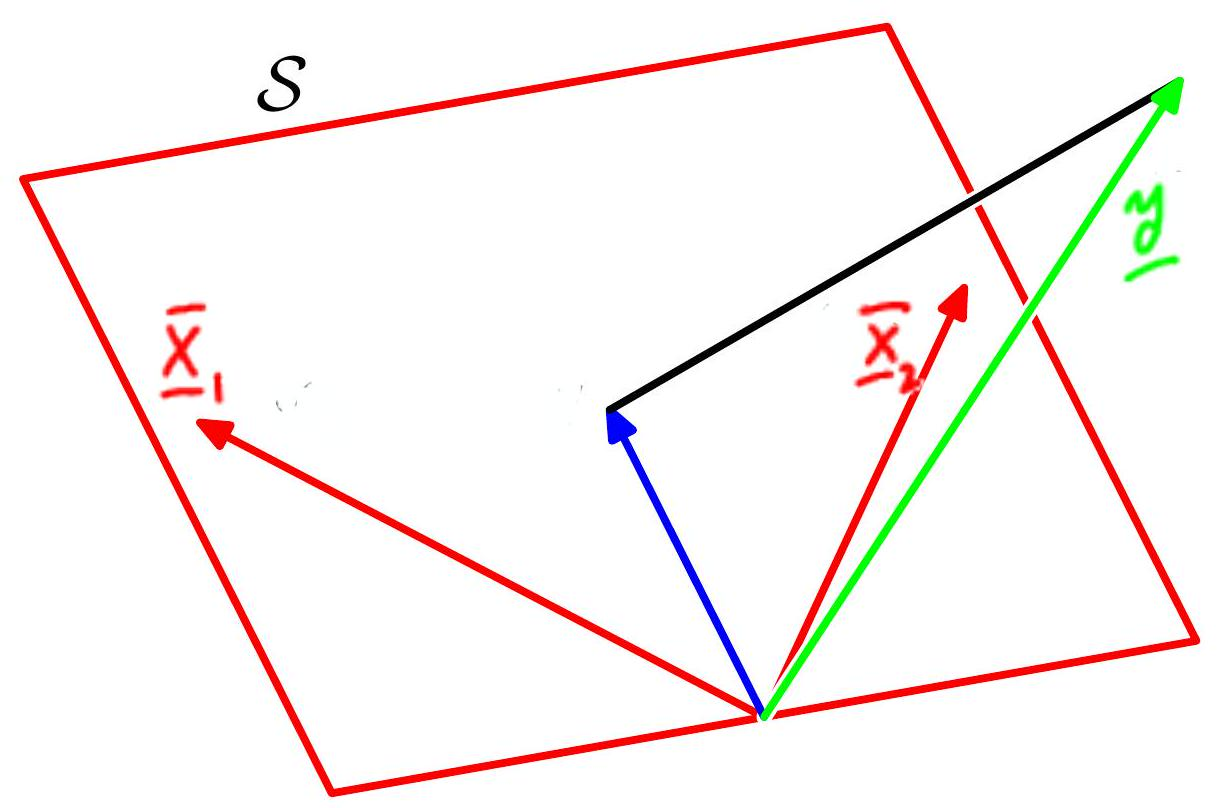
\includegraphics[max width=\textwidth]{2023_12_30_a01c196f804cf1b80331g-6}
\end{center}

\section*{Least Squares}
The matrix $\mathbf{X}^{\top} \mathbf{X} \in \mathbb{R}^{D \times D}$ is called the Gram matrix. If it is invertible, we can multiply the normal equation by the inverse of the Gram matrix from the left to get a closed-form expression for the minimum:

$$
\mathbf{w}^{\star}=\left(\mathbf{X}^{\top} \mathbf{X}\right)^{-1} \mathbf{X}^{\top} \mathbf{y}
$$

We can use this model to predict a new value for an unseen datapoint (test point) $\mathbf{x}_{m}$ :

$$
\hat{y}_{m}:=\mathbf{x}_{m}^{\top} \mathbf{w}^{\star}=\mathbf{x}_{m}^{\top}\left(\mathbf{X}^{\top} \mathbf{X}\right)^{-1} \mathbf{X}^{\top} \mathbf{y} .
$$

\section*{Invertibility and Uniqueness}
Note that the Gram matrix $\mathbf{X}^{\top} \mathbf{X} \in \mathbb{R}^{D \times D}$ is invertible if and only if $\mathbf{X}$ has full column rank, or in other words $\operatorname{rank}(\mathbf{X})=D$.

Proof: To see this assume first that $\operatorname{rank}(\mathbf{X})<D$. Then there exists a non-zero vector $\mathbf{u}$ so that $\mathbf{X u}=\mathbf{0}$. It follows that $\mathbf{X}^{\top} \mathbf{X u}=\mathbf{0}$, and so $\operatorname{rank}\left(\mathbf{X}^{\top} \mathbf{X}\right)<D$. Therefore, $\mathbf{X}^{\top} \mathbf{X}$ is not invertible.

Conversely, assume that $\mathbf{X}^{\top} \mathbf{X}$ is not invertible. Hence, there exists a non-zero vector $\mathbf{v}$ so that $\mathbf{X}^{\top} \mathbf{X v}=\mathbf{0}$. It follows that

$$
\mathbf{0}=\mathbf{v}^{\top} \mathbf{X}^{\top} \mathbf{X} \mathbf{v}=(\mathbf{X} \mathbf{v})^{\top}(\mathbf{X} \mathbf{v})=\|\mathbf{X} \mathbf{v}\|^{2}
$$

This implies that $\mathbf{X v}=\mathbf{0}$, i.e., $\operatorname{rank}(\mathbf{X})<D$.

\section*{Rank Deficiency and III-Conditioning}
Unfortunately, in practice, $\mathbf{X}$ is often rank deficient.

\begin{itemize}
  \item If $D>N$, we always have $\operatorname{rank}(\mathbf{X})<D$
\end{itemize}

(since row rank $=$ col. rank)

\begin{itemize}
  \item If $D \leq N$, but some of the columns $\mathbf{x}_{:}$are (nearly) collinear, then the matrix is illconditioned, leading to numerical issues when solving the linear system.
\end{itemize}

Can we solve least squares if $\mathbf{X}$ is rank deficient? Yes, using a linear system solver.

\section*{Summary of Linear Regression}
We have studied three types of methods:

\begin{enumerate}
  \item Grid Search

  \item Iterative Optimization Algorithms (Stochastic) Gradient Descent

  \item Least squares

\end{enumerate}

closed-form solution, for linear MSE

\section*{Additional Notes}
\section*{Closed-form solution for MAE}
Can you derive closed-form solution for 1-parameter model when using MAE cost function?

See this short article: \href{http://www}{http://www}. \href{http://johnmyleswhite.com/notebook/2013/03/}{johnmyleswhite.com/notebook/2013/03/} 22/modes-medians-and-means-an-unifying-perspective/.

\section*{Implementation}
There are many ways to solve a linear system, but using the QR decomposition is one of the most robust ways. Matlab's backslash operator and also NumPy's linalg package implement this in just one line:

$$
\mathrm{w}=\mathrm{np} . \operatorname{linalg} \cdot \operatorname{solve}(\mathrm{X}, \mathrm{y})
$$

For a robust implementation, see Sec. 7.5.2 of Kevin Murphy's book.


\end{document}